\documentclass{spisok-article}

\title{Использование обобщения теоремы Кёнига}

\newtheorem*{koenig}{Теорема (Кёниг)}}
\newtheorem*{koenig_ex}{Теорема (Обобщение теоремы Кёнига)}
\newtheorem*{example}{Пример}
\author{
  Захаров С.А.,
  студент кафедры вычислительной математики СПбГУ,
  serge.zakharov@mail.ru
  }


\begin{document}

\maketitle

\begin{abstract}
Теорема Кёнига, в различном виде часто упоминаемая в статьях и книгах по вычислительной математике - один из основных инструментов доказательства сходимости различных методов решения нелинейных уравнений: в большинстве своем, эти методы основаны на нахождении полюса обращенной функции нелинейного уравнения. \\
В плюсы к теоретической полезности теоремы также можно отнести и ее практическую силу - метод, прямиком основанный на теореме, позволяет довольно точно найти ближайший к исходной точке полюс.
\end{abstract}

\section{Введение}

Решение нелинейных уравнений, пусть и даже одной переменной - задача старая и популярная, так как решать её необходимо повсеместно. Огромное количество методов и идей может быть применено к данной задаче: как обобщения методов, разработанных для полиномов - например, метод Бернулли - так и сведение уравнения к виду, удобному для итераций, и решение его методами либо асимптотическими, либо с помощью теоремы Банаха о стационарной точке и теории голоморфных динамик. \\
Еще один тип методов естественно вытекает из простого обращения функции - вместо поиска нулей будем искать особые точки обращенной функции, нахождение которых, особенно в комплексной плоскости, имеет хорошее теоретическое обоснование: достаточно вспомнить об интегральной формуле Коши, известном поведении функции возле особых точек или о смысле радиуса сходимости ряда Тейлора (расстояние от центра до ближайшей особой точки).

\section{Обобщение теоремы Кёнига}
\subsection{Мотивировка и теоремы}
Самый простой метод последнего типа мотивирован признаком сходимости рядов Д'Аламбера - для него возникают вопросы в комплексном плане: можно ли каким-либо простым образом найти не только модуль особой точки, но и ее аргумент?\\
Это улучшение было получено в виде теоремы Кёнига\cite{house}:
\begin{koenig}
	Пусть\(f(z)\) - голоморфна в \(\mathbb{C}\) за исключением конечного числа особых точек \(Q = \{q_0, q_1, \dots, q_n\}\), упорядоченных по модулю и отделенных от нуля:  \(: |q_n| \geq |q_{n-1}|\geq \dots \geq |q_1| > |q_0| > 0 \). Тогда, если каждая особая точка из \(Q\) - простой полюс и ряд Тейлора функции в нуле имеет вид:
		\( f(z) = \sum\limits_{k=0}^{\infty}a_k z^k \), то ближайшую к нулю, по модулю, особую точку можно 	найти с помощью равенства: 
	\begin{displaymath}
		 \lim\limits_{n \to \infty}\frac{a_{n-1}}{a_{n}} = q_0.
	\end{displaymath}
\end{koenig}
С помощью других способов доказательства теоремы можно получить обобщение теоремы на случай кратных полюсов. Также, используя факт о том, что главная часть функции в соответствующей точке доминирует над всей остальной функцией, можно получить асимптотики:
\begin{koenig_ex}
	Пусть\(f(z)\) - голоморфна в \(\mathbb{C}\) за исключением конечного числа полюсов \(Q = \{q_0, q_1, \dots, q_n\}\), упорядоченных по модулю и отделенных от нуля:  \(: |q_n| \geq |q_{n-1}|\geq \dots \geq |q_1| >|q_0| > 0 \). Тогда, если ряд Тейлора функции в нуле имеет вид:
		\( f(z) = \sum\limits_{k=0}^{\infty}a_k z^k \), то верны равенства: 
	\begin{displaymath}
		 \lim\limits_{n \to \infty}\left|\frac{a_{n}}{a_{n-1}}\right| = \left|\frac{1}{q_0}\right|\left(1 + \frac{N-1}{n} + O\left(\left|\frac{q_0}{q_1}\right|^n\right)\right),
	\end{displaymath}
    \begin{displaymath}
		 \lim\limits_{n \to \infty}Arg\left(\frac{a_{n}}{a_{n-1}}\right) = Arg\left(\frac{1}{q_0}\right)\left(1 + O\left(\left|\frac{q_0}{q_1}\right|^n\right)\right),
	\end{displaymath}
	где \(N\) - кратность полюса \(q_0\).
\end{koenig_ex}
Стоит заметить, что условие о том, что лишь одна особая точка должна лежать на окружности радиуса сходимости, убрать никак нельзя. Это можно показать на простом примере:
\begin{example}
Возьмем какую-либо простую функцию с несколькими особыми  точками на окружности радиуса сходимости, например:
 \begin{displaymath}
 f(z) = \frac{1}{A-z} + \frac{1}{A+z} + \frac{1}{B-z}.
 \end{displaymath}
Зададим \(A\) и \(B\) так, чтобы \(|A|<|B|\). Покажем неудачу доказательства теоремы на данном примере. Легко посчитать, что коэффициент ряда Тейлора равен:
  \begin{displaymath}
 a_k = A^{-1-k} + (-1)^k A^{-1-k} + B^{-1-k} = A^{-1-k} \left( 1 + (-1)^k + \left(\frac{A}{B}\right)^{1+k} \right).
 \end{displaymath}
 Рассматривая отношение \(\frac{a_k}{a_{k-1}}\), беря частичный предел по нечетным индексам \(k\), получим \(\frac{A}{B}\). С другой стороны, для четных индексов отношение равно \(1\). Следовательно, предела не существует.
\end{example}
\subsection{Вычисление коэффициентов ряда Тейлора}
Из того, что изложено выше, ясно, что, все-таки, основную часть времени работы алгоритма должно занимать вычисление коэффициентов ряда Тейлора. Рассмотрим два метода:
\begin{enumerate}
\item Квадратурная формула для сильноосциллирующих функций \cite{bach}. \\
	Квадратуру следует использовать для интегральной формулы Коши производной \(f(z)\):
	 \begin{displaymath}
	 	a_n = \frac{1}{2 \pi i} \int\limits_{|z| = 1}\frac{f(z)}{z^{n+1}}dz = \int\limits_{-1}^{1}f(e^{-i \pi \phi})e^{i \pi \phi n}d\phi .
	 \end{displaymath}
	 Приблизим \(f(z)\) с помощью интерполяционного многочлена, за узлы возьмем корни \(n\)-го многочлена Лежандра, разложим интерполяционный многочлен по многочленам Лежандра:
	\begin{displaymath}
	f(x) \approx L_n(x) = \sum_{k=0}^{n}c_k P_k(x).
	\end{displaymath}
Домножая приближенное равенство на экспоненту нужной частоты и интегрируя, получим квадратуру:
	\begin{displaymath}
	\int\limits_{-1}^{1} e^{i \phi x}f(x) dx \approx \sum_{k=0}^{n}c_k \int\limits_{-1}^{1} e^{i \phi x}P_k(x) dx.
	\end{displaymath}
	Интегралы справа следует считать по интегрированным рекуррентным соотношениям, а коэффициенты \(c_k\) удобно находить с помощью классической формулы Гаусса. \\
	В данном виде формула очень неустойчива для больших частот экспоненты, но, можно заметить, что при делении отрезка интегрирования на \(k\) частей сама частота делится на \(k\), а при сдвиге отрезка интегрирования весь интеграл домножается на определенную константу - помимо, конечно, изменения самой функции под интегралом. Из этого вытекает возможность использования составной квадратурной формулы.
\begin{example}
	Разбивая отрезок интегрирования на \(S\) частей, для \(22\)го коэффициента функции \(f(x) = \frac{1}{1-0.3 x}\), который приближенно равен \(a_{22} \approx 3.138102 \cdot 10^{-12}\), получим:
		\center{\begin{tabular}{| c | c | }
					\hline \(S\) & \(a_{22}\) \\
  					\hline \(1\)& \(2.083256 \cdot 10^{10}\) \\
  					\hline \(2\) & \(7.437875 \cdot 10^{-5}\) \\
  					\hline \(3\) & \(7.681297 \cdot 10^{-11}\) \\
  					\hline \(4\) & \(3.069000 \cdot 10^{-12}\) \\
  					\hline \(5\) & \(3.135116 \cdot 10^{-12}\) \\
  					\hline \(6\) & \(3.138055 \cdot 10^{-12}\) \\
  					\hline
				\end{tabular}}\\
	Вычисления выполнены при \(16\)ти верных знаках, на каждом промежутке было взято \(100\) точек.
\end{example}
\item Метод, основанный на приближении оператора обратного сдвига \cite{bsa}. \\
	Сам же оператор, рассматриваемый над пространством последовательностей \(l^2\), выглядит как:
  	\begin{displaymath}
 		Ba : (a_0, a_1, a_2, \dots) \to (a_1, a_2, a_3, \dots).
 	\end{displaymath}
	Для нас интересен оператор над голоморфными на единичном круге функциями, аналогичный этому. Ввести его можно как:
	\begin{displaymath}
 		Bf : f(z) \to \frac{f(z)-f(0)}{z}.
 	\end{displaymath}
 	Ясно, что если \(f(z) = a_0 + a_1 z + \dots\), то
 	\begin{displaymath}
 		B^kf(0) = a_k.
 	\end{displaymath}
 	Пусть фиксирована какая-либо квадратура на единичной окружности, выбраны соответствующие ей точки. Также, даны значения \(f(z)\) в этих точках. На основе этих значений, вычислим \(f(0)\) с помощью интегральной формулы Коши, посчитаем оператор обратного сдвига в фиксированных точках на окружности. Выполняя эти действия многократно, получим нужный \(a_n\).
\begin{example}
	Взяв квадратуру левых прямоугольников по \(N\) точкам, для \(22\)го коэффициента функции \(f(x) = \frac{1}{1-0.3 x}\), приближенно равному \(a_{22} \approx 3.138102 \cdot 10^{-12}\), получим: \\
	\center{\begin{tabular}{| c | c | }
					\hline \(N\) & \(a_{22}\) \\
  					\hline \(10\)& \( 1.124676 \cdot 10^{-21}\) \\
  					\hline \(20\) & \(1.729928 \cdot 10^{-16}\) \\
  					\hline \(30\) & \(3.138102 \cdot 10^{-12}\) \\
  					\hline \(40\) & \(3.138119 \cdot 10^{-12}\) \\
  					\hline \(50\) & \(3.138100 \cdot 10^{-12}\) \\
  					\hline \(60\) & \(3.138101 \cdot 10^{-12}\) \\
  					\hline
	\end{tabular}}\\
	Вычисления выполнены при \(16\)ти верных знаках.
\end{example}
\end{enumerate}
Ясно, что вычисление быстро убывающих коэффициентов довольно сложно выполнить с нужной точностью. Это сильно влияет на точность самого метода.
\begin{example}
	Для функции из примеров выше, n отвечает \(\frac{a_n}{a_{n-1}}\):
		\center{\begin{tabular}{| c | c | c | }
			\hline \(n\)  & Приближение сдвига &   Квадратура   \\
  			\hline \(22\) &   \( 0.30000107\)  & \(0.29999705\) \\
  			\hline \(24\) &   \( 0.29999130\)  & \(0.30000829\) \\
  			\hline \(26\) &   \( 0.30007641\)  & \(0.30101691\) \\
  			\hline \(28\) &   \( 0.29835943\)  & \(0.30121857\) \\
  			\hline \(30\) &   \( 0.30468013\)  & \(2.77276067\) \\
  			\hline
		\end{tabular}}\\
\end{example}
Видно, что метод на основе второй квадратуры выходит более требовательным даже на таком простом примере.
\subsection{Ускорение сходимости}
Заметим, что в асимптотике модуля присутствует \(\frac{1}{n}\) - член, довольно сильно замедляющий сходимость для кратных полюсов. Избавимся от него с помощью простой линейной комбинации:
	\begin{displaymath}
				c_k = \left|\frac{a_{k}}{a_{k-1}}\right| = \left|\frac{1}{q_0}\right|\left( 1+ \frac{N-1}{k} + O\left(\left|\frac{q_0}{q_1}\right|^k\right)\right), \\
\end{displaymath}
\begin{displaymath}		
		2 \cdot c_{2k} - c_{k} =  \left|\frac{1}{q_0}\right|\left( 1+  O\left(\left|\frac{q_0}{q_1}\right|^k\right)\right).
	\end{displaymath}
	Выигрыш легко виден:
\begin{example}
			Для функции \(f(z) = \left(\frac{3}{1-0.5 z}\right)^{10} + \left(\frac{1}{1-0.4 z}\right)^4 + \exp(x)\), график зависимости найденного модуля от номера члена последовательности, используется алгоритм на основе второй квадратуры. Заметьте, что для неускоренной последовательности, ради честности сравнения, нечетные члены пропускаются.	
			\center {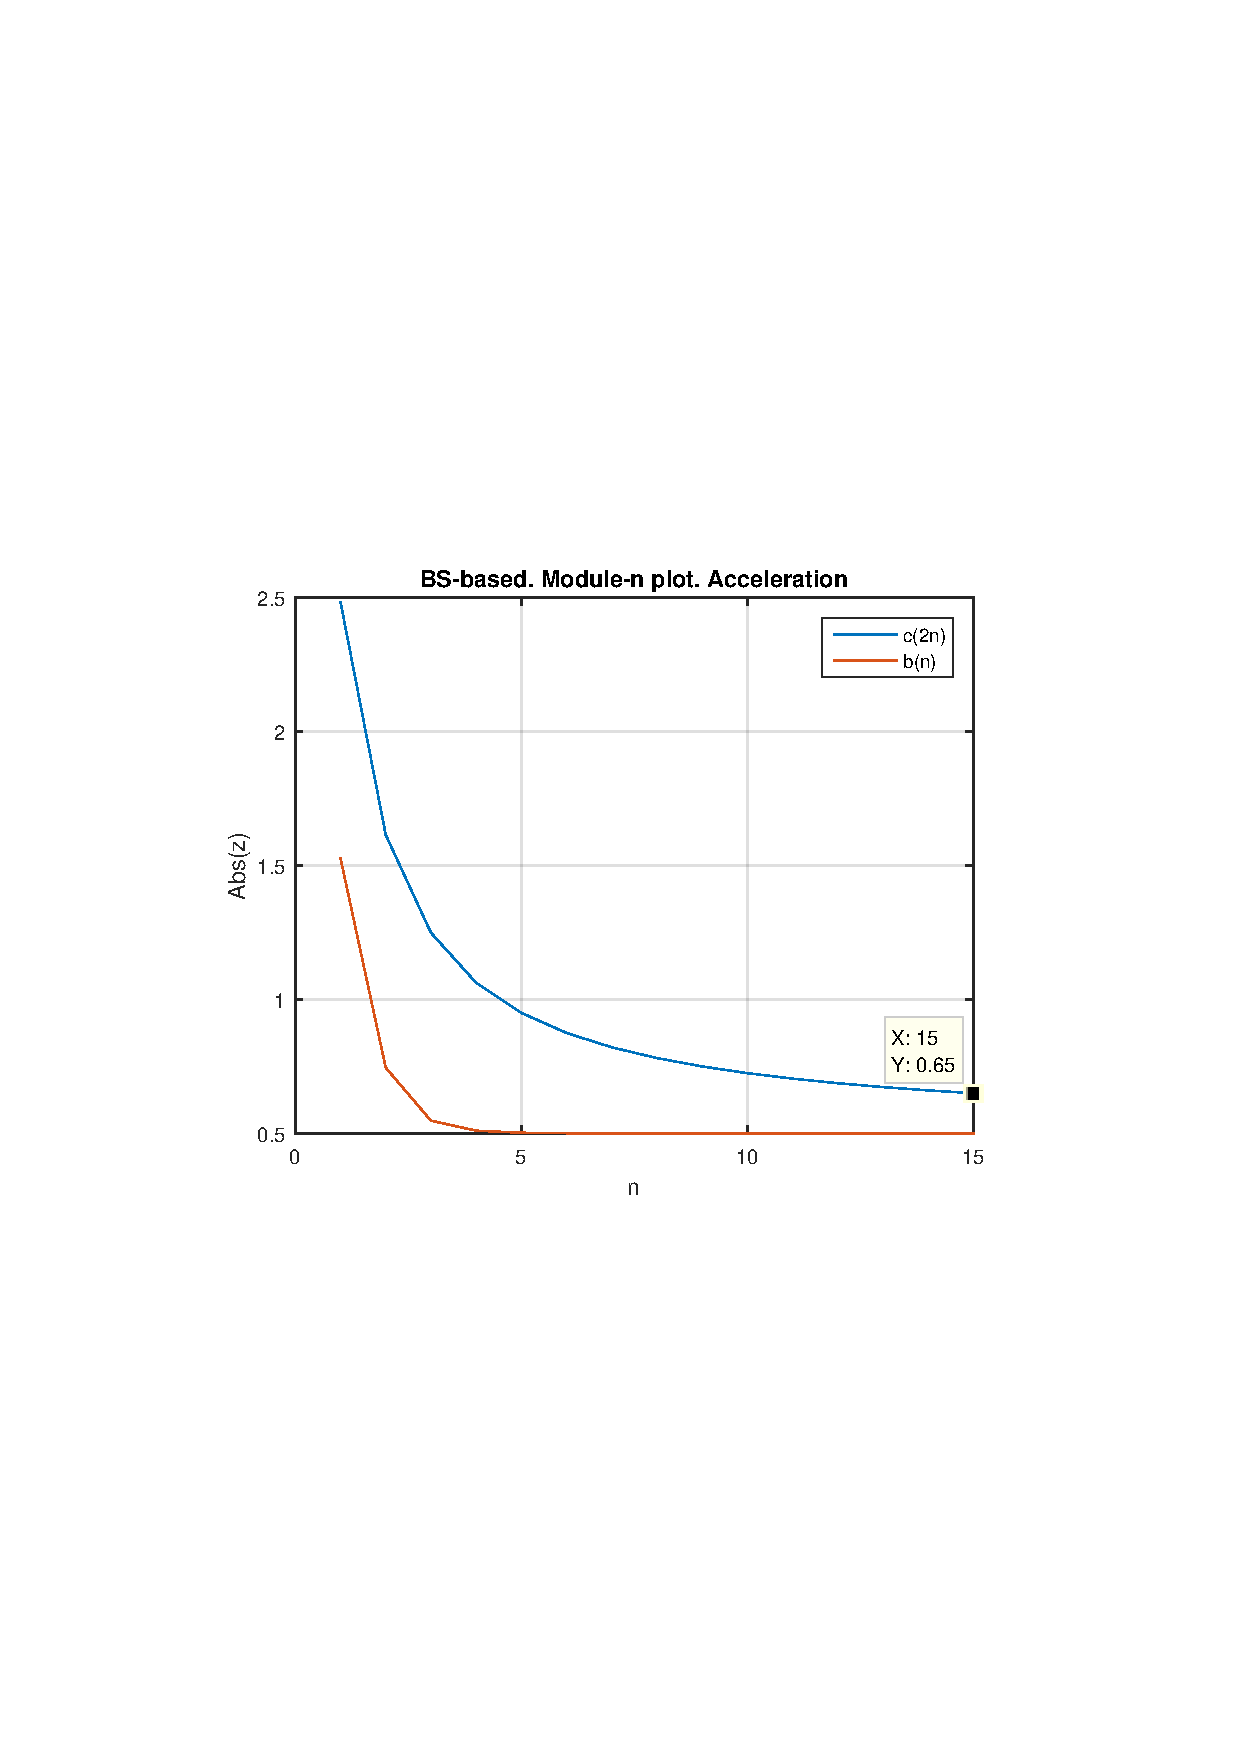
\includegraphics[trim={0cm 9cm 0 9.5cm},clip, width=0.9\linewidth]{bs-based_module-plot_accel.pdf} }
\end{example}
Также, легко показать, что на сходимость аргумента данное ускорение никак не влияет:
\begin{example}
			Для функции \(f(z) = \frac{3}{1-i \cdot 0.5 z} + \frac{1}{1-0.4 z} + \exp(x) \), график зависимости найденного модуля от номера члена последовательности, используется алгоритм на основе второй квадратуры.	
			\center {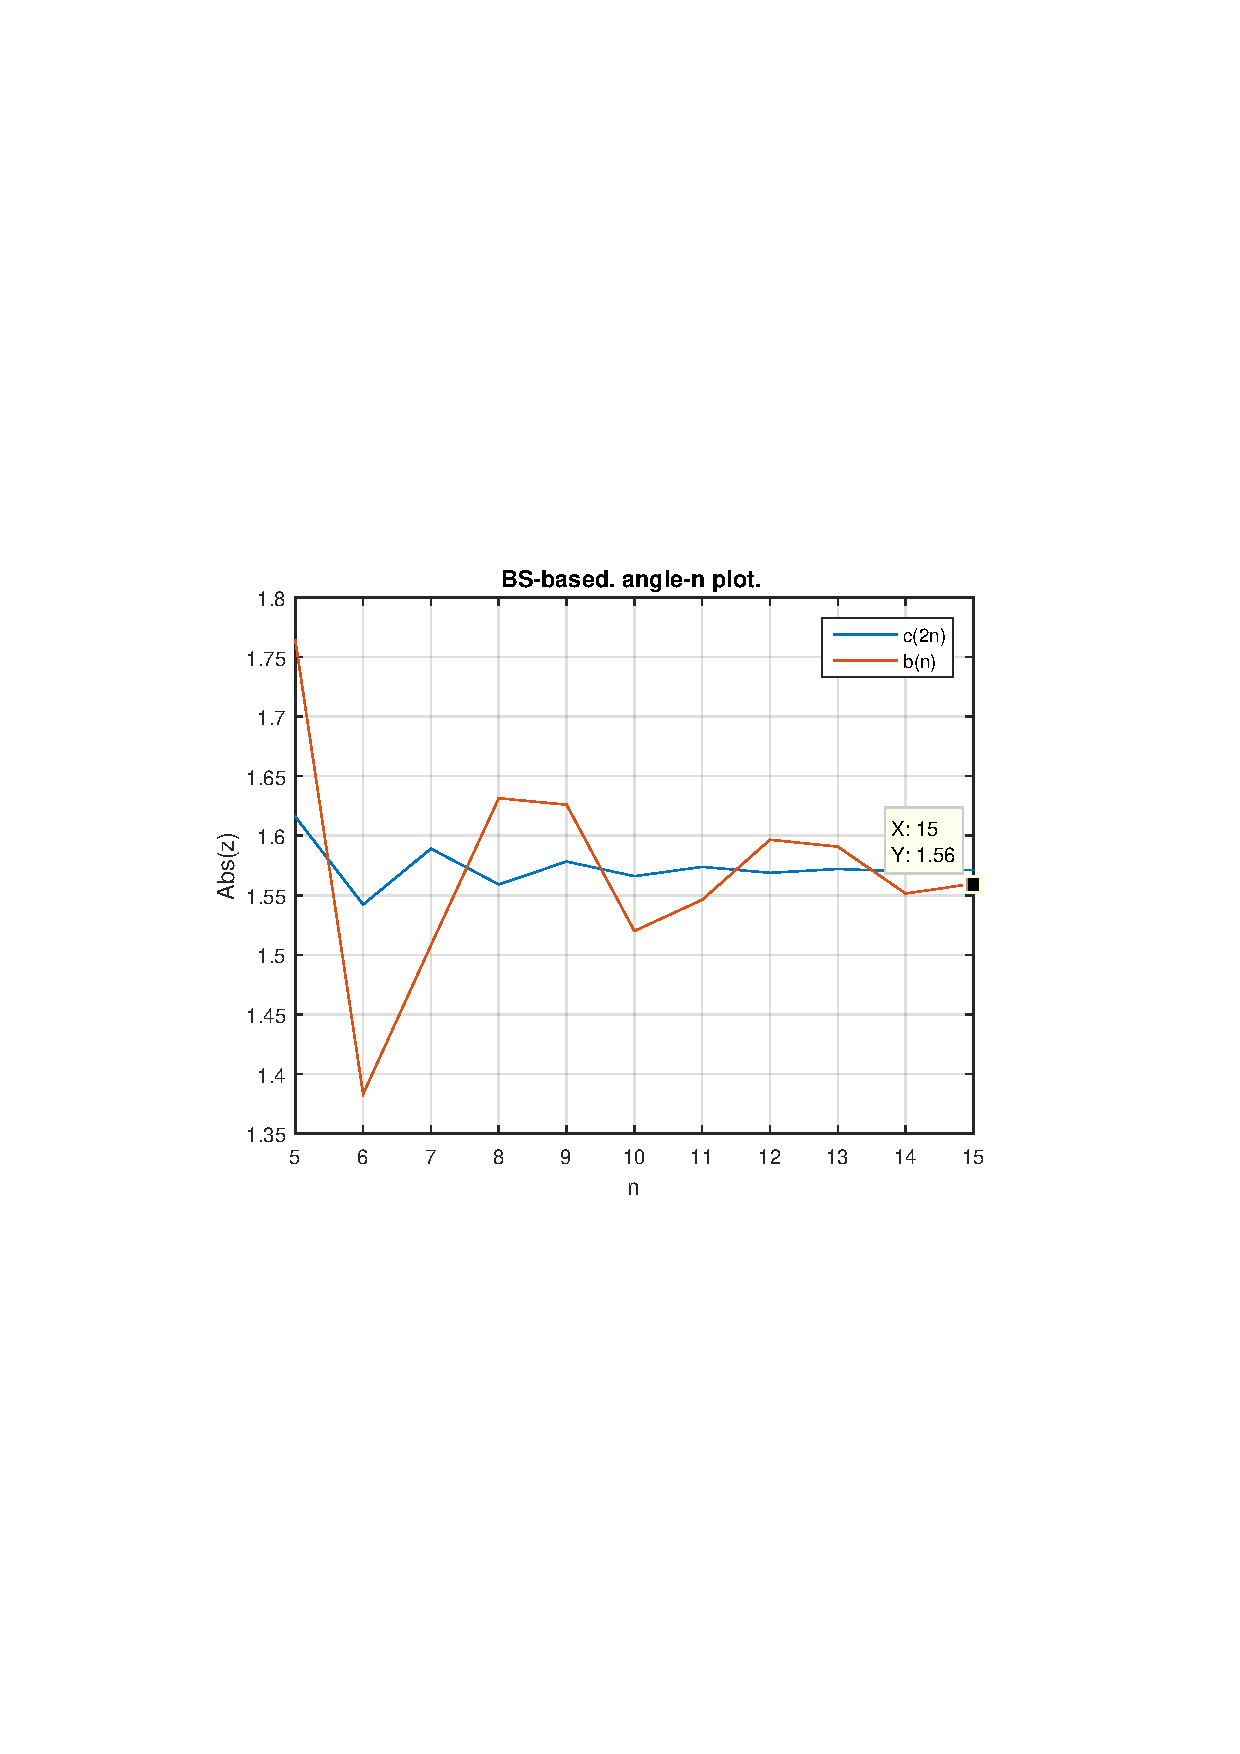
\includegraphics[trim={0cm 9cm 0 9.5cm},clip, width=0.9\linewidth]{bs-based_angle-plot.pdf} }
\end{example}
\subsection{Использование}
Пусть мы достигли какого-то значения с помощью нашего метода. Попробуем сдвинуться на найденное, тем самым подойдя ближе к нужному полюсу. В итоге, к сожалению, тем самым мы сильно уменьшим производные главной части, и метод начнет вести себя неустойчиво:
\begin{example} Для функции \(f(z) = \frac{3}{1-0.5 z} + \left(\frac{1}{1-0.4 z}\right)^3 + \exp(x)\). Сдвинем нашу функцию на заранее найденное значение: \(g(z) = f(z + 0.5104^{-1})\). По значениям метода, на основе второй квадратуры, построим график модуля:
\center {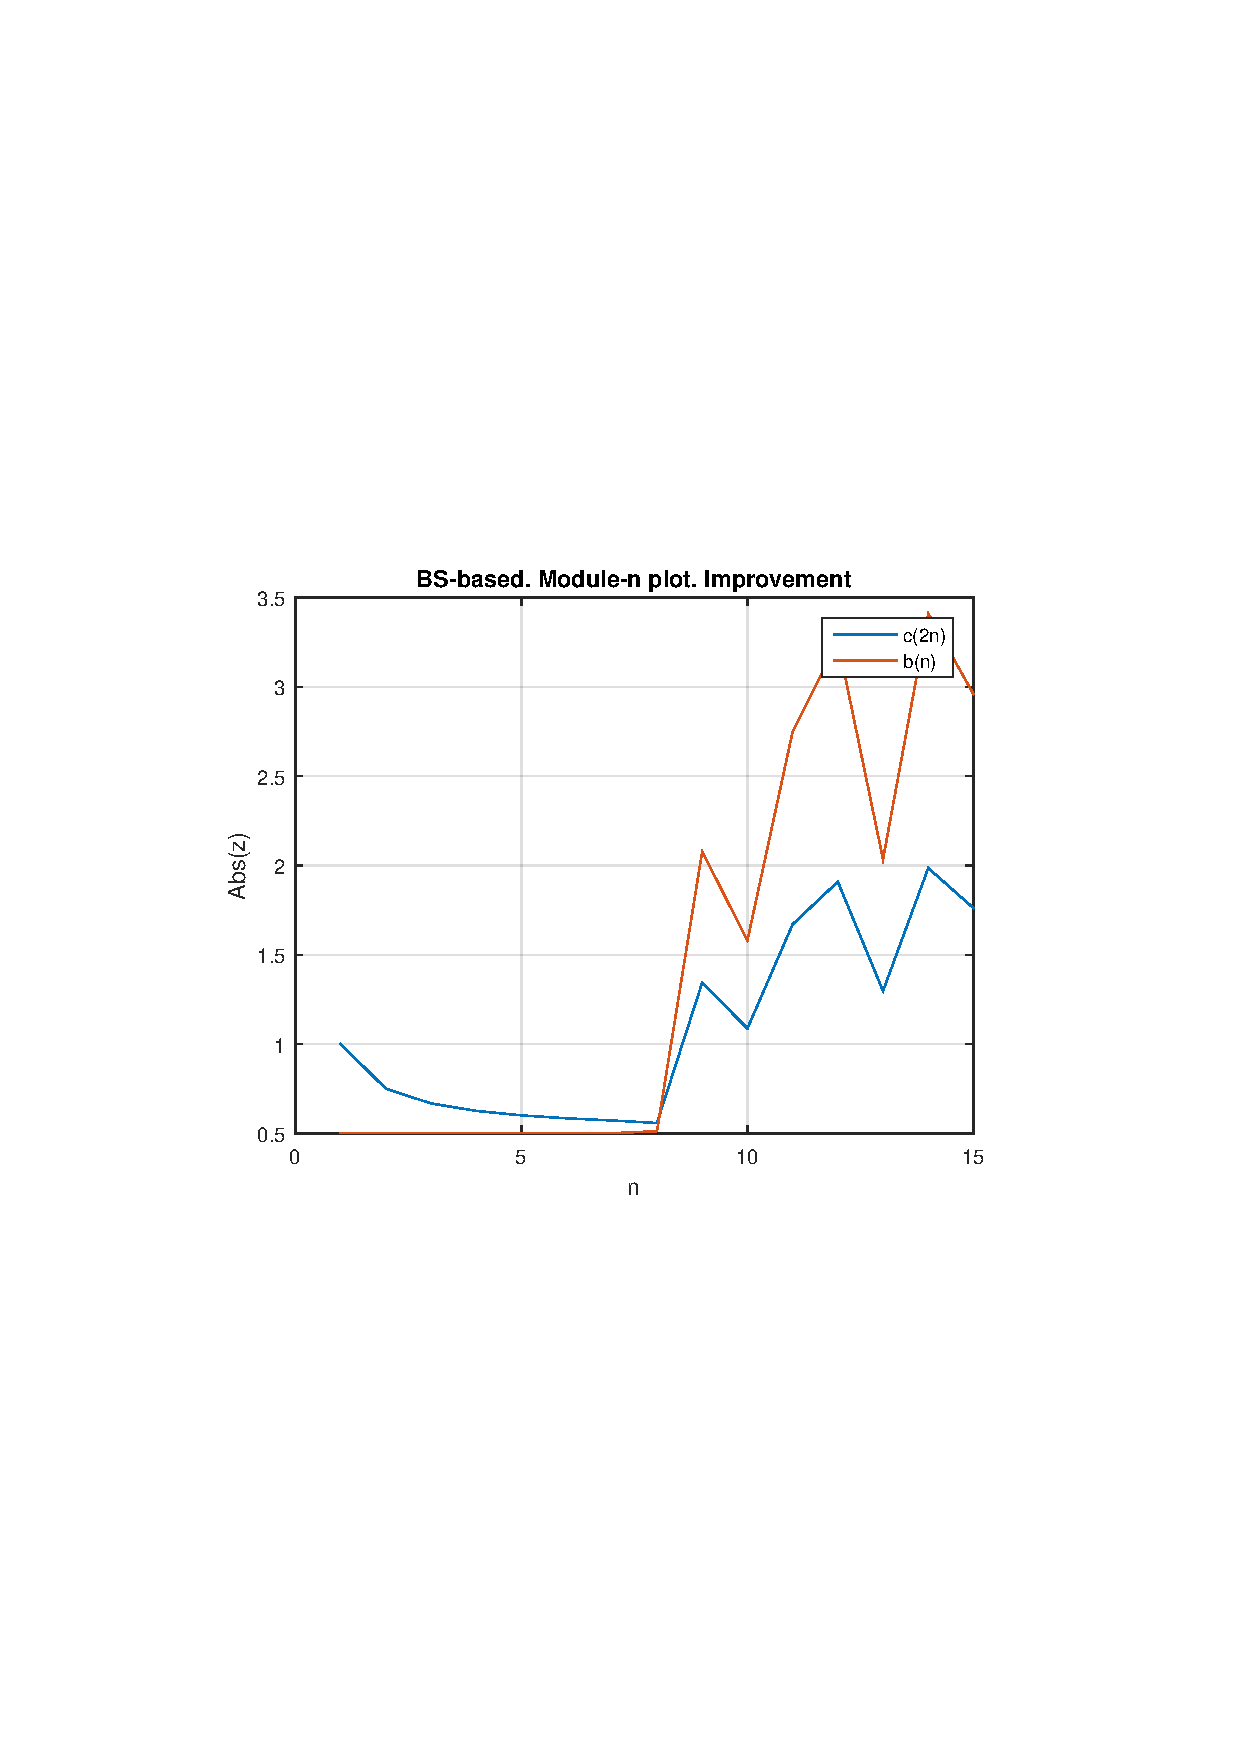
\includegraphics[trim={0cm 9cm 0 9.5cm},clip, width=0.9\linewidth]{bs-based_module-plot_improvement.pdf} }
\end{example}
Поэтому, видимо, для дальнейшего уточнения следует использовать методы другого типа.
\section{Дальнейшее}
Метод довольно прост и имеет множество недостатков, но его идеи были переняты другими, более удобными и современными методами. Так, по подобию доказательства Кёнига, A. S. Householder построил обобщенную теорему для одновременного нахождения нескольких особых точек функции. Ускорив последовательности, он получил метод Айткена\cite{house} и QD-алгоритм для нахождения полюсов\cite{henrici}.   \\
С помощью обобщения, полученного Хаусхолдером, при известном количестве полюсов функции, легко показать сходимость аппроксимаций Паде фиксированного деноминатора. Это наводит на мысль о том, что использовать их и другие сходящиеся к ним рациональные приближени, для нахождения полюсов было бы вполне разумно. \\
Следующий метод нахождения полюсов рациональных функций был изложен китайскими математиками Wen Mi и Tao Qian в их совместной статье 2014 года, основан на свойствах оператора обратного сдвига над пространством \(H_2(\mathbb{D})\) Харди-2  от единичного круга. Его описание можно найти в \cite{bsa}.
\section{Заключение}
В данной статье были описаны методы решения нелинейных уравнений, основанные на нахождении особых точек обращенной функции, детально разобран на примерах метод, основанный на теореме Кёнига, обсуждается ускорение его сходимости, его использование. Также, с помощью примеров сравниваются два алгоритма нахождения коэффициентов ряда Тейлора голоморфной в круге функции.

\renewcommand\refname{Литература}
\begin{thebibliography}{8}
\bibitem{house} Householder A. S. The Numerical Treatment of a Single Nonlinear Equation //
  McGraw-Hill, 1970. ---
  С. 122.

\bibitem{bsa} Wen Mi, Tao Qian. On backward shift algorithm for estimating poles of systems // 
  Automatica, Volume 50, Issue 6, June 2014. ---
  С. 1603–1610.
  
\bibitem{bach} Бахвалов Н. С., Васильева Л. Г. Вычисление интегралов от осциллирующих функций при помощи интерполяции по узлам квадратур Гаусса // 
  Ж. вычисл. матем. и матем. физ., 1968, T. 8, № 1. ---
  С. 175–181.

\bibitem{henrici} Henrici P. Applied and Computational Complex Analysis //
  John Wiley \& Sons, 1988 ---
  С. 608
\end{thebibliography}

\end{document}
